\documentclass[12pt]{article}
\usepackage[margin=2.5cm]{geometry}
\usepackage{enumerate}
\usepackage{amsfonts}
\usepackage{amsmath}
\usepackage{fancyhdr}
\usepackage{amsmath}
\usepackage{amssymb}
\usepackage{amsthm}
\usepackage{mdframed}
\usepackage{graphicx}
\usepackage{subcaption}
\usepackage{adjustbox}
\usepackage{listings}
\usepackage{xcolor}
\usepackage{booktabs}
\usepackage[utf]{kotex}

\definecolor{codegreen}{rgb}{0,0.6,0}
\definecolor{codegray}{rgb}{0.5,0.5,0.5}
\definecolor{codepurple}{rgb}{0.58,0,0.82}
\definecolor{backcolour}{rgb}{0.95,0.95,0.92}

\lstdefinestyle{mystyle}{
    backgroundcolor=\color{backcolour},
    commentstyle=\color{codegreen},
    keywordstyle=\color{magenta},
    numberstyle=\tiny\color{codegray},
    stringstyle=\color{codepurple},
    basicstyle=\ttfamily\footnotesize,
    breakatwhitespace=false,
    breaklines=true,
    captionpos=b,
    keepspaces=true,
    numbers=left,
    numbersep=5pt,
    showspaces=false,
    showstringspaces=false,
    showtabs=false,
    tabsize=1
}

\lstset{style=mystyle}

\begin{document}
\title{CSC148 Worksheet 13 Solution}
\author{Hyungmo Gu}
\maketitle

\section*{Question 1}
\begin{enumerate}[a.]
    \item

    The following diagram tells us the stopping condition occurs when both
    \textit{curr1} and \textit{curr2} is \textit{None}.

    \begin{center}
    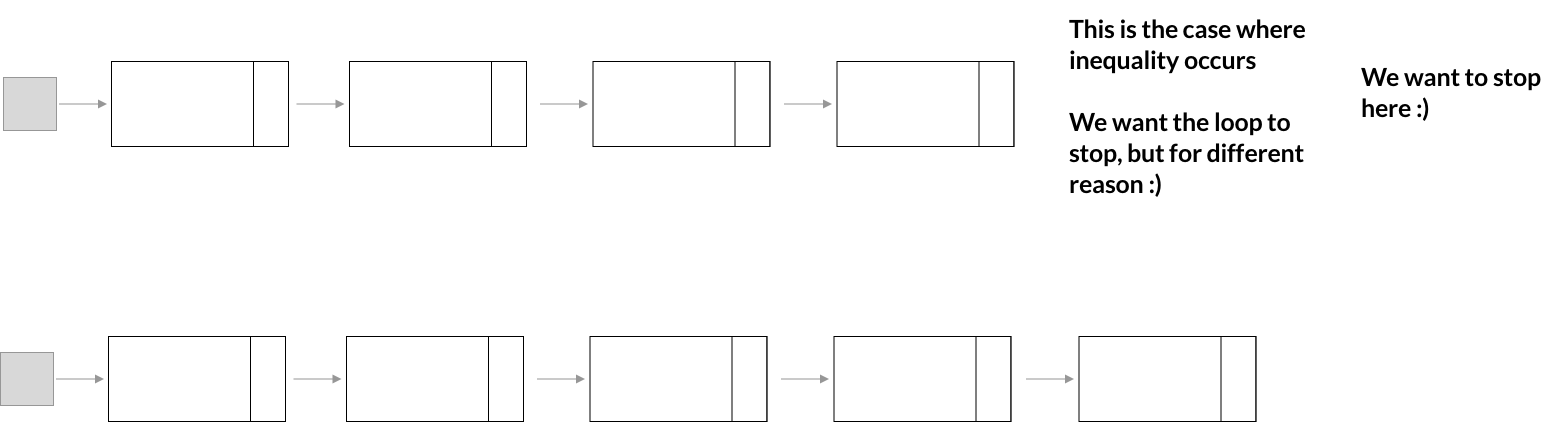
\includegraphics[width=\linewidth]{images/worksheet_13_q1a_solution.png}
    \end{center}

    \bigskip

    Using this fact, the python expression involving \textit{curr1}
    and \textit{curr2} that expresses the stopping condition is

    \bigskip

    \begin{lstlisting}[language=Python]
    (curr1 is not None) and (curr2 is not None)
    \end{lstlisting}

    \item

    Python expression for the while loop condition is

    \begin{lstlisting}[language=Python]
    while (curr1 is not None) and (curr2 is not None):
        ...
    \end{lstlisting}

    \item

    The code for traversing two list is

    \begin{lstlisting}[language=Python]
    while (curr1 is not None) and (curr2 is not None):
        if curr1 is None or curr2 is None:
            return False

        if curr1.item != curr2.item:
            return False

        curr1 = curr1.next
        curr2 = curr2.next
    \end{lstlisting}

\end{enumerate}

\section*{Question 2}



\end{document}